\subsection{Alternative to Estimate $\hat{\textbf{A}}$}  
As concluded the Cov-DL algorithm do not recover a sufficient estimate of the mixing matrix $\mathbf{A}$, therefore a different approach is necessary. 

Replacing the insufficient estimate by a fixed estimate $\hat{\mathbf{A}}_{\text{fix}}$ is one immediately solution. 
This choice is supported by the observations from Cov-DL2 where $\mathbf{A}_{\text{ini}}$ matrix provides an estimate which is happens to be a least as good as the one provided by Cov-DL. 
Thus the challenge is now to determine a fixed matrix for which its characteristics resembles those of the true mixing matrix. 
However, from chapter \ref{ch:motivation} it is clear that no specific characteristic of the mixing matrix is known, which supports the choice of an random matrix of Gaussian distribution or similar, as it was chosen for the initial guess for the estimate.   
From this perspective three fixed mixing matrices are defined, by drawing each entry from a specified distribution: 
\begin{itemize}
\item[] $\hat{\textbf{A}}_{uni}\sim \mathcal{U}(-1,1)$
\item[] $\hat{\textbf{A}}_{norm}\sim \mathcal{N}(0, 2)$ 
\item[] $\hat{\textbf{A}}_{gauss}\sim \mathcal{N}(0,1)$                                           
\end{itemize}

Note that the third matrix $\hat{\textbf{A}}_{gauss}$ is generated the same way as the true mixing matrix of the stochastic data sets. thus it is expected to have the lowest MSE when compared to the true $\textbf{A}$. However, it is of interest to investigate whether is the best estimate of $\textbf{A}$ which provide the best estimate of $\textbf{X}$.   

A different option regarding a fixed estiamtion of $\textbf{A}$ is to utilize the ICA algorithm, described in appendix \ref{app:ICA}. By the ICA algorithm it is possible to solve the EEG inverse problem for both $\textbf{A}$ and $\textbf{X}$, in the case where $k \leq M$.
Consider a simulation of a stochastic data set specified by $N = k = M$. Solving the system by ICA yields an estimate of $\textbf{A}$. Now reduce the data set $\textbf{Y}$ such that $M \leq k$. Similar the estimate of $\textbf{A}$ is reduced by removing the same rows as in $\textbf{Y}$, this yields the an estimate $\hat{\textbf{A}}_{ICA}$ which can be used as a fixed input to M-SBL along with the corresponding reduced $\textbf{Y}$.

The four different fixed estimates $\hat{\mathbf{A}}$ are tested on stochastic data sets specified by $M = 10$, $N = k = 16$ and $L = 1000$. 
To get the average performance 50 different simulations are conducted with the same specifications, each system $\textbf{X}$ is estimated from each of the four fixed estimates of $\textbf{A}$\footnote{note that for each of the 50 repetitions  four new $\hat{\textbf{A}}_{\text{fix}}$ are fixed}, and the MSE is are computed. The resulting averaged $MSE_{\textbf{A}}$ and $MSE_{\textbf{X}}$ are visualised  in figure \ref{fig:vary_A}, for each of the four $\hat{\mathbf{A}}_{\text{fix}}$. 
Furthermore, the plotted values are found in table \ref{tab:fixed}.

\begin{figure}[H]
\centering
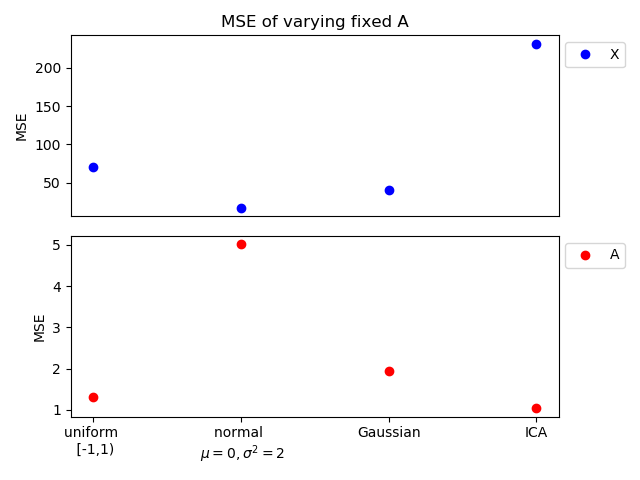
\includegraphics[scale=0.5]{figures/ch_6/A_fix.png}
\caption{Plot of average MSE for each of the four $\hat{\mathbf{A}}_{\text{fix}}$ resulting from a stochastic data set specified by $M=10$, $N=k=16$ and $L=1000$.}
\label{fig:vary_A}
\end{figure}
\noindent

\begin{table}[H]
\centering
\begin{tabular}{|c|c|c|c|c|}
\hline
 & $\hat{\textbf{A}}_{uni}$ & $\hat{\textbf{A}}_{norm}$	 & $\hat{\textbf{A}}_{gauss}$ & $\hat{\textbf{A}}_{ICA}$ \\
\hline
MSE$_\mathbf{A}$ & 1.330 & 4.907 & 1.976 & 1.060 \\
\hline
MSE$_\mathbf{X}$ & 89.70 & 21.33 & 35.93 & 148.0 \\
\hline
\end{tabular}
\caption{Average MSE values resulting from stochastic data set specified by $M=10$, $N=k=16$ and $L=1000$ with a fixed estimate $\hat{\mathbf{A}}_{\text{fix}}$.}
\label{tab:fixed}
\end{table}

From table \ref{tab:fixed} and figure \ref{fig:vary_A} it is first of all seen that relation between the MSE of $\textbf{A}$ and $\textbf{X}$ is not as expected, as the lowest $\textbf{A}_{MSE}$ results in the highest $\textbf{X}_{MSE}$ and so forth. The lowest $\textbf{A}_{MSE}$ is achieved by using $\hat{\mathbf{A}}_{\text{fix}}$, which confirms that the ICA algorithm manage to estimate $\textbf{A}$ when $k\leq M$. However, as this do not result in the best estimate of $\textbf{X}$ a different choice of $\hat{\textbf{A}}$ is still considered. The lowest $\textbf{X}_{MSE}$ is achieved by use of $\hat{\textbf{A}}_{norm}$, which resulted in the largest $\textbf{A}_{MSE}$. 
      
As the main interest in this thesis is to identify and localise the active sources of EEG measurement a low $\textbf{X}_{mse}$ is more desirable than a low $\textbf{A}_{mse}$. Furthermore, a disadvantage of using $\hat{\textbf{A}}_{ICA}$ is the limitations in practise when $k=M$ i not possible.     
From these observation a fixed estimate of the mixing matrix drawn from a normal distribution with mean 0 and variance 2, $\hat{\textbf{A}}_{norm}$, is chosen as the the alternative estimate of $\textbf{A}$, and is used throughout the thesis. 


